\chapter{Basic Concepts}
% \label{ch:basic-concepts}

\section{Introduction}
\begin{definition}[Distributed]
   Spreading tasks and resources across multiple machines or locations
\end{definition}

Distribution enhances resilience and efficiency through decentralization.

\begin{example}
   Google's global data centers ensuring users across the world get fast search results.
\end{example}

\begin{definition}[Scalable]
   Ability to grow and handle increasing workload without compressing performance
\end{definition}

Scaling is about growth and expansion while maintaining efficiency

\begin{example}
   Netflix scaling its services to accommodate millions of users streaming content simultaneously
\end{example}

\section{Scalability and Motivations}
Scalability refers to a system's ability to handle increased load by adding resources (e.g., servers, nodes, or storage).
{Typically we have to two types of scalability:\ns
\begin{itemize}
   \item \textbf{Vertical} - Adding resources to a single node
   \item \textbf{Horizontal} - Adding more nodes to a system
\end{itemize}}

In relation to scalability, systems can hence be characterized by \textbf{performance}, intended as the ability to handle a growing number of requests, and \textbf{elasticity}, intended as the ability to scale up or down based on current needs.
On this matter, scalability may come in two flavours:
\begin{itemize}
   \item \textbf{Strong Scalability} - The system's performance increases linearly with the number of resources.
   \note{This is ideal for systems where the workload can be evenly distributed across many nodes}
   \item \textbf{Weak Scalability} - The system's performance does not degrade as the number of users increases
   \note{This fits best systems where the total workload grows alongside the system's resources}
\end{itemize}

\subsection{But why? - Motivation for Scalable Distributed Systems}
\begin{itemize}
   \item \textbf{Growing data} - large datasets from applications like social media, IoT, AI, etc.
   \item \textbf{Global Users} - Billions of users worldwide
   \item \textbf{Performance} - Reducing latency, increasing throughput, and improving reliability
   \note{\ul{Sometimes latency is \textit{not} a priority}: in some systems it is okay to have high latency to guarantee high throughput and reliability}
\end{itemize}

The challenges are mostly to \textbf{manage resources} across geographically distributed systems, and ensuring \textbf{low latency} and \textbf{high availability}.

\subsection{Target Architectures}
Some architectures which require scalable distributed systems are IoT networks, High-Performance Computing (HPC), and Cloud/Edge Computing.

\framedt{Example - Cameras in a district}{
   {\centering What if I send all the data gathered from cameras to a \textit{single cloud}?}
   \labelitemize{\textit{Pros}}{
      \begin{itemize}
         \item Unlimited storage and processing power
         \item Centralized management
         \item Simplicity
      \end{itemize}
   }
   \labelitemize{\textit{Cons}}{
      \begin{itemize}
         \item High latency
         \item High bandwidth usage
         \item Single point of failure (Scalability and Reliability)
      \end{itemize}
   }
}

{But also simpler applications may considerably benefit from scalable and distributed architectures.\ns
\begin{itemize}
   \item Large graph analysis
   \item Stream processing
   \item Streaming services
   \item Machine Learning
   \item Big Data
   \item Computational Fluid Dynamics
   \item Web and online services
\end{itemize}}

\subsubsection{Parallel computing}
\textit{Can't we rely on parallel computing to solve these problems?}\\
Not really, parallel fits different needs and works in a slightly different way.
\begin{figure}[htbp]
   \centering
   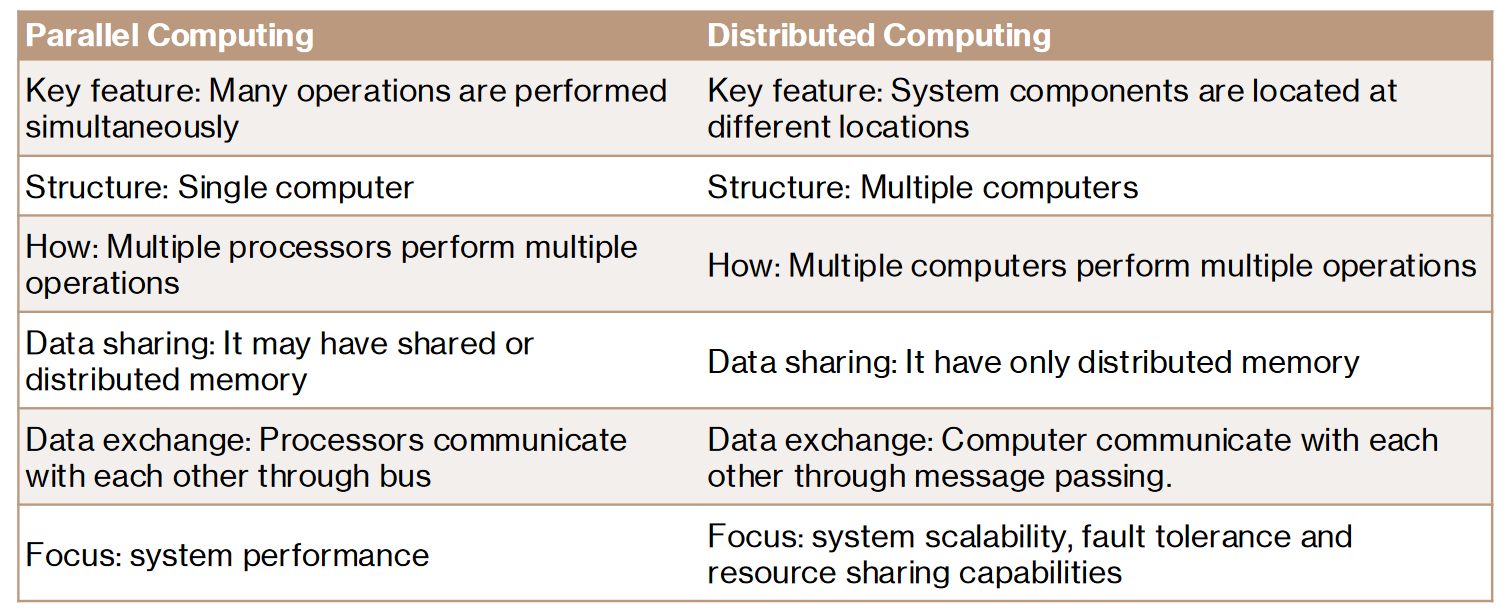
\includegraphics{images/01/parallel.png}
   \caption{From Parallel to Distributed}
   \label{fig:01/parallel}
\end{figure}

\subsection{Distribution is cool, but\dots}

Consider that local computation is always faster than remote computation. (\textit{Waaay faster})\\
From the CPU perspective, time passes \textit{very slowly} when the data travels outside the machine.
\note{If one CPU cycle happened every second, sending a packet in a data center would take 20 hours.
Sending it from NY to San Francisco would take 7 years.}

\section{Assessment Method - Exam}
There are three options, but note that
\textbf{\ul{in every case an oral exam will follow}.}
\begin{enumerate}
   \item \textit{Writing a Survey or a Report}
   students can conduct a comprehensive survey or prepare an in-depth report on a topic or technology related to the course.
   \item \textit{Individual or Group Project} ($leq 3$ members)
   Designing, implementing and presenting a solution or prototype related to scalable distributed computing.
   \item \textit{Traditional Written Exam}
   ``Questions, answers\dots you know the drill.''
   Very sad option, in my opinion, but prof. Dazzi did not completely discourage it.
\end{enumerate}
Prof. Dazzi is very open to proposals for the exam, he'd like to stimulate our creativity and curiosity.

Prof. Dazzi says that usually its oral examinations last from 30 to 35 minutes, even though there may be exceptions.\\
Clearly, if the student chooses the report or the project, part of the oral will be about the proposed work, but also questions about the course will be asked.